\documentclass[border=3pt]{standalone}
\usepackage[T1]{fontenc}
\usepackage[utf8]{inputenc}
\usepackage{lmodern}
\usepackage{amsmath,amssymb}
\usepackage{tikz}
\usetikzlibrary{arrows.meta}

\definecolor{mattercol}{HTML}{35678A}
\definecolor{gaugecol}{HTML}{AD742C}
\definecolor{supercol}{HTML}{833A65}
\definecolor{inkcol}{HTML}{222630}
\definecolor{outcol}{HTML}{3A576A}

\begin{document}
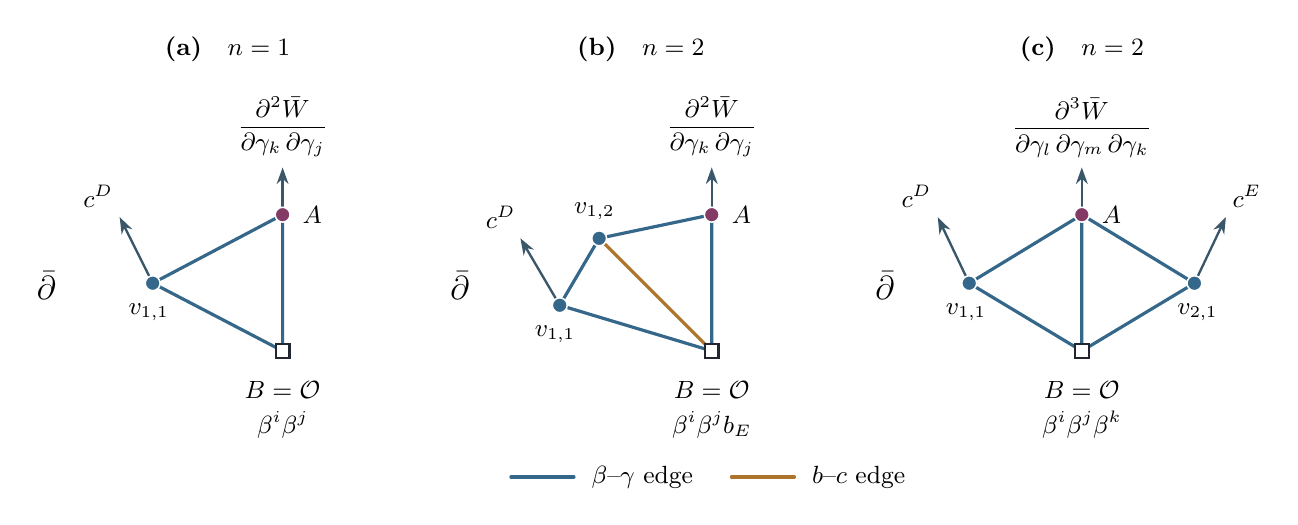
\begin{tikzpicture}[
  x=1cm, y=1cm, font=\small,
  medge/.style={draw=mattercol, line width=1.15pt, line cap=round},
  gedge/.style={draw=gaugecol, line width=1.15pt, line cap=round},
  outarr/.style={draw=outcol, line width=0.85pt, -{Stealth[length=2.1mm, width=1.5mm]}, shorten <=2.2pt},
  mnode/.style={circle, fill=mattercol, draw=white, line width=0.55pt, inner sep=1.9pt},
  snode/.style={circle, fill=supercol, draw=white, line width=0.55pt, inner sep=1.9pt},
  inode/.style={rectangle, fill=white, draw=inkcol, line width=0.85pt, inner sep=2.5pt}
]

% ---------------- Panel (a): n = 1 ----------------
\begin{scope}[xshift=0cm]
  \node[font=\small] at (1.95, 4.55) {\textbf{(a)}\quad $n=1$};
  \node[font=\large] at (-0.35, 1.55) {$\bar\partial$};

  \coordinate (A)  at (2.65, 2.45);
  \coordinate (B)  at (2.65, 0.72);
  \coordinate (v1) at (1.00, 1.58);

  \draw[medge] (v1)--(A) (v1)--(B) (A)--(B);
  \draw[outarr] (A) -- (2.65, 3.05);
  \draw[outarr] (v1) -- (0.58, 2.42);

  \node[snode] at (A) {};
  \node[mnode] at (v1) {};
  \node[inode] at (B) {};

  \node[anchor=west] at (2.78, 2.45) {$A$};
  \node[anchor=north] at (0.95, 1.44) {$v_{1,1}$};
  \node[anchor=south] at (2.65, 3.06) {$\dfrac{\partial^2\bar W}{\partial\gamma_k\,\partial\gamma_j}$};
  \node[anchor=south east] at (0.62, 2.42) {$c^D$};

  \node at (2.65, 0.22) {$B=\mathcal O$};
  \node at (2.65, -0.22) {$\beta^i\beta^j$};
\end{scope}

% ---------------- Panel (b): n = 2 ----------------
\begin{scope}[xshift=5.25cm]
  \node[font=\small] at (1.95, 4.55) {\textbf{(b)}\quad $n=2$};
  \node[font=\large] at (-0.35, 1.55) {$\bar\partial$};

  \coordinate (A)  at (2.85, 2.45);
  \coordinate (B)  at (2.85, 0.72);
  \coordinate (v2) at (1.42, 2.15);
  \coordinate (v1) at (0.92, 1.30);

  \draw[medge] (v1)--(v2) (v2)--(A) (v1)--(B) (A)--(B);
  \draw[gedge] (v2)--(B);
  \draw[outarr] (A) -- (2.85, 3.05);
  \draw[outarr] (v1) -- (0.42, 2.15);

  \node[snode] at (A) {};
  \node[mnode] at (v1) {};
  \node[mnode] at (v2) {};
  \node[inode] at (B) {};

  \node[anchor=west] at (2.98, 2.45) {$A$};
  \node[anchor=north] at (0.86, 1.16) {$v_{1,1}$};
  \node[anchor=south] at (1.36, 2.26) {$v_{1,2}$};
  \node[anchor=south] at (2.85, 3.06) {$\dfrac{\partial^2\bar W}{\partial\gamma_k\,\partial\gamma_j}$};
  \node[anchor=south east] at (0.48, 2.15) {$c^D$};

  \node at (2.85, 0.22) {$B=\mathcal O$};
  \node at (2.85, -0.22) {$\beta^i\beta^j b_E$};
\end{scope}

% ---------------- Panel (c): n = 2 ----------------
\begin{scope}[xshift=10.65cm]
  \node[font=\small] at (2.15, 4.55) {\textbf{(c)}\quad $n=2$};
  \node[font=\large] at (-0.35, 1.55) {$\bar\partial$};

  \coordinate (A)  at (2.15, 2.45);
  \coordinate (B)  at (2.15, 0.72);
  \coordinate (v1) at (0.72, 1.58);
  \coordinate (v2) at (3.58, 1.58);

  \draw[medge] (v1)--(A) (v2)--(A) (v1)--(B) (v2)--(B) (A)--(B);
  \draw[outarr] (A) -- (2.15, 3.05);
  \draw[outarr] (v1) -- (0.32, 2.42);
  \draw[outarr] (v2) -- (3.98, 2.42);

  \node[snode] at (A) {};
  \node[mnode] at (v1) {};
  \node[mnode] at (v2) {};
  \node[inode] at (B) {};

  \node[anchor=west] at (2.28, 2.45) {$A$};
  \node[anchor=north] at (0.68, 1.44) {$v_{1,1}$};
  \node[anchor=north] at (3.62, 1.44) {$v_{2,1}$};
  \node[anchor=south] at (2.15, 3.06) {$\dfrac{\partial^3\bar W}{\partial\gamma_l\,\partial\gamma_m\,\partial\gamma_k}$};
  \node[anchor=south east] at (0.36, 2.42) {$c^D$};
  \node[anchor=south west] at (3.94, 2.42) {$c^E$};

  \node at (2.15, 0.22) {$B=\mathcal O$};
  \node at (2.15, -0.22) {$\beta^i\beta^j\beta^k$};
\end{scope}

% ---------------- Legend ----------------
\begin{scope}[yshift=-0.88cm]
  \draw[medge] (5.55, 0) -- (6.35, 0);
  \node[anchor=west] at (6.45, 0) {$\beta\text{--}\gamma$ edge};
  \draw[gedge] (8.35, 0) -- (9.15, 0);
  \node[anchor=west] at (9.25, 0) {$b\text{--}c$ edge};
\end{scope}

\end{tikzpicture}
\end{document}
